\documentclass[a4paper,UTF8]{ctexart}
\usepackage{graphicx}
\usepackage{geometry}
\usepackage{xcolor}
\usepackage{amsmath}
\usepackage{enumerate}
\usepackage{caption}
\usepackage{listings}
\usepackage{array}
\usepackage{booktabs}
\usepackage{tikz}
\usetikzlibrary{shapes,arrows}
\usepackage{pgfplots}
\pgfplotsset{compat=1.17}
\usepackage{appendix}
\captionsetup[lstlisting]{labelfont=bf,justification=justified}
\usepackage{multicol}
\setlength{\columnsep}{3em}
\usepackage{float}

\graphicspath{{img/}}

\usepackage[colorlinks,linkcolor=blue]{hyperref}
\usepackage{bookmark}
\providecommand{\code}[2]{\lstinputlisting[language=#2,caption=\href{run:#1}{\ttfamily #1}]{#1}}
\providecommand{\img}[1]{\includegraphics[width=0.88\textwidth]{#1}}

% listings
\definecolor{grey}{rgb}{0.8,0.8,0.8}
\definecolor{darkgreen}{rgb}{0,0.3,0}
\definecolor{darkblue}{rgb}{0,0,0.3}
\lstset{%
    numbers=left, %行号
    numberstyle=\scriptsize\color{grey},
    showstringspaces=false,
    showspaces=false,%
    tabsize=4,%
    frame=shadowbox,%
    basicstyle={\ttfamily\normalsize},%
    keywordstyle=\color{blue!80!black}\bfseries,%
    identifierstyle=,%
    commentstyle=\color{green!50!blue}\itshape,%
    stringstyle=\color{green!50!black},%
    rulesepcolor=\color{gray!20!white},
    breaklines,
    columns=flexible,
    extendedchars=false,
    %mathescape=true,
    language=verilog,
}

\begin{document}
\title{\normalsize \underline{计算机系统结构实验}\\\LARGE 实验 3 报告\\\vspace*{1em}\normalsize 简单的类 MIPS 单周期处理器\\部件实现--控制器,ALU}
\author{李子龙\\ 518070910095}
\date{\today}
\maketitle
\tableofcontents
\clearpage

\section{实验目的}

\begin{enumerate}
    \item 理解 CPU 控制器,ALU 的原理
    \item 主控制器 Ctr 的实现
    \item 运算单元控制器 ALUCtr 的实现
    \item ALU 的实现
    \item 使用功能仿真
\end{enumerate}

\section{原理分析}

\subsection{主控制器单元模块 Ctr}

\begin{figure}[h]
    \centering
    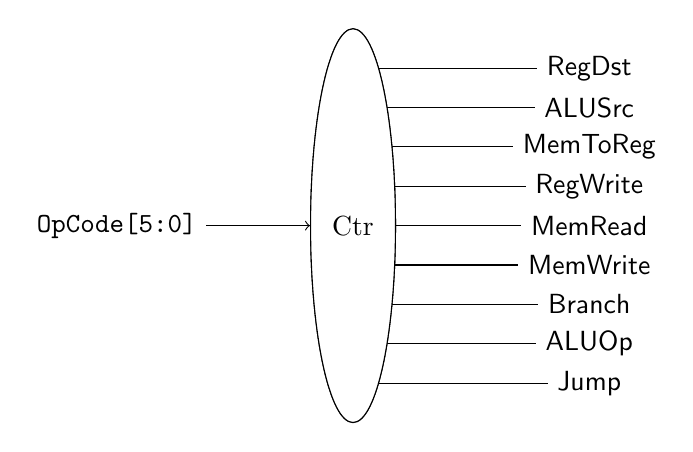
\begin{tikzpicture}

\node [ellipse,draw,minimum height=5cm,fill=white] (v2) at (0,0) {Ctr};
\node [font=\ttfamily] (v1) at (-3,0) {OpCode[5:0]};

\draw  (v1) edge[->] (v2);
\node[font=\sffamily] (v3) at (3,2) {RegDst};
\node[font=\sffamily] (v4) at (3,1.5) {ALUSrc};
\node[font=\sffamily] (v5) at (3,1) {MemToReg};
\node[font=\sffamily] (v6) at (3,0.5) {RegWrite};
\node[font=\sffamily] (v7) at (3,0) {MemRead};
\node[font=\sffamily] (v8) at (3,-0.5) {MemWrite};
\node[font=\sffamily] (v9) at (3,-1) {Branch};
\node[font=\sffamily] (v10) at (3,-1.5) {ALUOp};
\node[font=\sffamily] (v11) at (3,-2) {Jump};

\foreach \x in {3,...,11}
    \draw (v2) |- (v\x);

\node [ellipse,draw,minimum height=5cm,fill=white] at (0,0) {Ctr};

\end{tikzpicture}
    \caption{主控制器单元模块}
\end{figure}

主控制器单元对输入指令 \verb"Instruction[31:26]" (即 \verb"opCode" 部分)译码。指令与对应的 \verb"opCode" 对应列表于表 \ref{tab:opcode}。

\begin{table}[h]
    \centering
    \caption{指令操作码表}
    \label{tab:opcode}
    \begin{tabular}{>{\ttfamily}l>{\ttfamily}c}
        \toprule
        指令 & opCode \\
        \midrule
        R: add,sub,and,or,slt & 000000 \\
        I: lw & 100011 \\
        I: sw & 101011 \\
        I: beq & 000100 \\
        J: j & 000010 \\
        \bottomrule
    \end{tabular}
\end{table}

译码完成后,需要针对对应的针脚输出对应的值,输出参数表如表 \ref{tab:ctr} 所示。

\begin{table}
    \centering
    \caption{主控制模块真值表}
    \label{tab:ctr}
    \begin{tabular}{>{\sffamily}l>{\ttfamily}c>{\ttfamily}c>{\ttfamily}c>{\ttfamily}c>{\ttfamily}c}
        \toprule
        信号名 & R & lw & sw & beq & j \\
        \midrule
        RegDst      & 1 & 0 & X & X & X \\
        ALUSrc      & 0 & 1 & 1 & 0 & X \\
        MemToReg    & 0 & 1 & X & X & X \\
        RegWrite    & 1 & 1 & 0 & 0 & 0 \\
        MemRead     & 0 & 1 & 0 & 0 & 0 \\
        MemWrite    & 0 & 0 & 1 & 0 & 0 \\
        Branch      & 0 & 0 & 0 & 1 & 0 \\
        ALUOp       & 10 & 00 & 00 & 01 & XX \\
        Jump        & 0 & 0 & 0 & 0 & 1 \\
        \bottomrule
    \end{tabular}
\end{table}

\subsection{算术逻辑单元控制器模块 ALUCtr}

\begin{figure}[h]
    \centering
    \begin{tikzpicture}

\node [ellipse,draw,minimum height=3cm,fill=white] (v2) at (0,0) {ALUCtr};
\node [font=\ttfamily] (v1) at (-3,0) {funct[5:0]};
\node [font=\sffamily] (v3) at (0,-3) {ALUOp[1:0]};
\node [font=\sffamily] (v4) at (3,0) {aluCtrOut[3:0]};

\draw (v1) edge[->] (v2);
\draw (v3) edge[->] (v2);
\draw (v2) edge[->] (v4);

\end{tikzpicture}
    \caption{ALUCtr 模块}
\end{figure}

算术逻辑单元控制器模块(ALUCtr)根据主控制器(Ctr)传来的 \verb"ALUOp" 来判断指令类型,并根据 \verb"Instruction[5:0]"(即 \verb"funct")来判断指令类型。并通过 \verb"altCtrOut[3:0]" 输出对应信号。对应列表列于表 \ref{tab:aluctr}。

\begin{table}[h]
    \centering
    \caption{ALUCtr 输入输出关系}
    \label{tab:aluctr}
    \begin{tabular}{>{\ttfamily}ll>{\ttfamily}c>{\ttfamily}cl>{\ttfamily}c}
        \toprule
        指令 & 详细指令 & ALUOp & funct & ALU 操作 & altCtrOut \\
        \midrule
        lw & load word & 00 & XXXXXX & add & 0010 \\
        sw & store word & 00 & XXXXXX & add & 0010 \\
        beq & branch equal & 01 & XXXXXX & subtract & 0110 \\
        R & add & 10 & 100000 & add & 0010 \\
        R & sub & 10 & 100010 & subtract & 0110 \\
        R & and & 10 & 100100 & and & 0000 \\
        R & or & 10 & 100101 & or & 0001 \\
        R & slt & 10 & 101010 & set less than & 0111 \\
        \bottomrule
    \end{tabular}
\end{table}

\subsection{ALU 模块}

\begin{figure}[H]
    \centering
    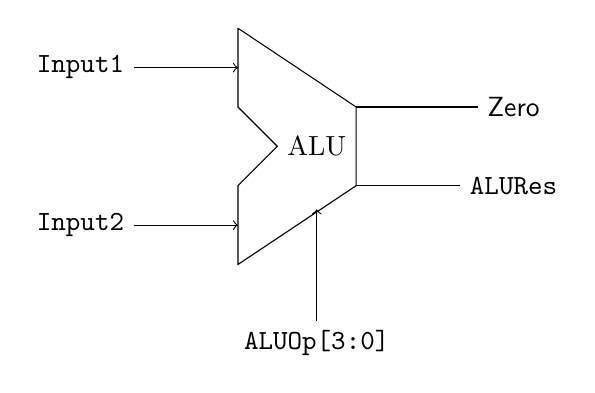
\begin{tikzpicture}

\draw (-1,1.5) -- (-1,0.5) -- (-0.5,0) -- (-1,-0.5) -- (-1,-1.5) -- (0.5,-0.5) node (v5) {} -- (0.5,0.5) node (v3) {} -- (-1,1.5);
\node at (0,0) {ALU};
\node[font=\ttfamily] (v1) at (-3,1) {Input1};
\node[font=\ttfamily] (v2) at (-3,-1) {Input2};
\draw (v1) edge[->] (-1,1);
\draw (v2) edge[->] (-1,-1);
\node[font=\sffamily] (v4) at (2.5,0.5) {Zero};
\draw  (0.5,0.5) edge (v4);
\node[font=\ttfamily] (v6) at (2.5,-0.5) {ALURes};
\draw  (0.5,-0.5) edge (v6);
\node[font=\ttfamily] (v7) at (0,-2.5) {ALUOp[3:0]};
\draw (v7) edge[->] (0,-0.8);
\end{tikzpicture}
    \caption{ALU 模块}
\end{figure}

ALU 模块对输入 \verb"Input1" 和 \verb"Input2" 进行数值运算。\verb"ALUOp[3:0]" 将会指定操作模式,并输出为 \verb"ALURes",\verb"Zero" 将指示结果是否为 0。操作模式与对应功能列于表 \ref{tab:alu}。

\begin{table}[H]
    \centering
    \caption{ALU 操作}
    \label{tab:alu}
    \begin{tabular}{>{\ttfamily}cc}
        \toprule
        ALUOp & 功能 \\
        \midrule
        0000 & 按位和 \\
        0001 & 按位或 \\
        0010 & 和 \\
        0110 & 减 \\
        0111 & 小于则设定 \\
        1100 & 按位或非 \\
        \bottomrule
    \end{tabular}
\end{table}

\section{代码实现}

\subsection{主控制模块 Ctr}

使用了 case 语句判断对应的 \verb"opCode" 以输出。例如对于 R 型语句:
\begin{lstlisting}[language=verilog,caption=Ctr.v]
    always @(opCode) begin
        case (opCode)
            6'b000000:      // R type
            begin
                RegDst      = 1;
                ALUSrc      = 0;
                MemToReg    = 0;
                RegWrite    = 1;
                MemRead     = 0;
                MemWrite    = 0;
                Branch      = 0;
                ALUOp       = 2'b10;
                Jump        = 0;
            end
            //...
        endcase
    end
\end{lstlisting}

其余的部分对照表 \ref{tab:ctr} 编写。

\subsection{算术逻辑单元控制器模块 ALUCtr}

结合 \verb"aluOp" 和 \verb"funct" 编码,使用 case 语句判断,并根据表 \ref{tab:aluctr} 输出。
\begin{lstlisting}[language=verilog,caption=ALUCtr.v]
module ALUCtr(
    input [5:0] funct,
    input [1:0] aluOp,
    output [3:0] aluCtrOut
    );

    reg [3:0] ALUCtrOut;

    always @(aluOp or funct) begin
        casex ({aluOp, funct})
            8'b00xxxxxx:    ALUCtrOut = 4'b0010;
            8'bx1xxxxxx:    ALUCtrOut = 4'b0110;
            8'b1xxx0000:    ALUCtrOut = 4'b0010;
            8'b1xxx0010:    ALUCtrOut = 4'b0110;
            8'b1xxx0100:    ALUCtrOut = 4'b0000;
            8'b1xxx0101:    ALUCtrOut = 4'b0001;
            8'b1xxx1010:    ALUCtrOut = 4'b0111;
            default:        ALUCtrOut = 4'b1111;
        endcase
    end
    
    assign aluCtrOut = ALUCtrOut;
endmodule
\end{lstlisting}

\subsection{ALU 模块}

按照表 \ref{tab:alu} 构建 case 语句。注意 \verb"slt" 采用符号数比较(事实上 \verb"sltu" 是无符号数比较)。
\begin{lstlisting}[language=verilog,caption=ALU.v]
always @(input1 or input2 or aluCtr) begin
    case (aluCtr)
        4'b0010: ALURes = input1 + input2;
        4'b0110: ALURes = input1 - input2;
        4'b0000: ALURes = input1 & input2;
        4'b0001: ALURes = input1 | input2;
        4'b0111: begin          // slt
            if($signed(input1) < $signed(input2))
                ALURes = 1;
            else ALURes = 0; 
        end
        4'b1100: ALURes = ~(input1 | input2);
        default: ALURes = 0;
    endcase
    if(ALURes == 0)
        Zero = 1;
    else
        Zero = 0;
end
\end{lstlisting}

\section{仿真结果}

\subsection{主控制模块 Ctr}

主控制模块的激励信号如下所示。
\begin{lstlisting}[language=verilog,caption={Ctr\_tb.v}]
initial begin
    OpCode = 0;
    #100;
    #100 OpCode = 6'b000000;
    #100 OpCode = 6'b100011;
    #100 OpCode = 6'b101011;
    #100 OpCode = 6'b000100;
    #100 OpCode = 6'b000010;
    #100 OpCode = 6'b010101;
end
\end{lstlisting}

仿真结果如图 \ref{fig:ctr} 所示。对照表 \ref{tab:ctr} 可得信号一致。
\begin{figure}[H]
    \centering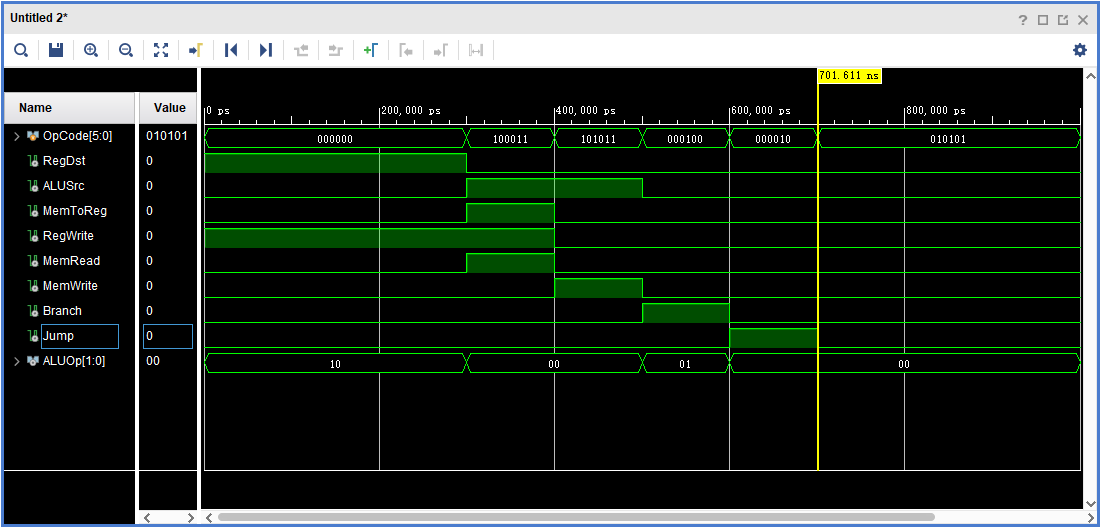
\includegraphics[width=\textwidth]{figure1.png}\caption{Ctr 仿真波形}\label{fig:ctr}
\end{figure}

\subsection{算术逻辑单元控制器模块 ALUCtr}

算术逻辑单元控制器模块的激励信号如下所示。

\begin{multicols}{2}
\begin{lstlisting}[language=verilog,caption={ALUCtr\_tb.v}]
initial begin
    Funct = 0;
    ALUOp = 0;
    #100;

    #100;
    Funct = 6'b000000;
    ALUOp = 2'b00;
    
    #100;
    Funct = 6'b000000;
    ALUOp = 2'b01;

    #100;
    Funct = 6'b000000;
    ALUOp = 2'b10;

    #100;
    Funct = 6'b000010;
    ALUOp = 2'b10;

    #100;
    Funct = 6'b000100;
    ALUOp = 2'b10;

    #100;
    Funct = 6'b000101;
    ALUOp = 2'b10;

    #100;
    Funct = 6'b001010;
    ALUOp = 2'b10;
    
end
\end{lstlisting}
\end{multicols}

激励结果如图 \ref{fig:aluctrtb} 所示。结果与表 \ref{tab:aluctr} 一致。
\begin{figure}
    \centering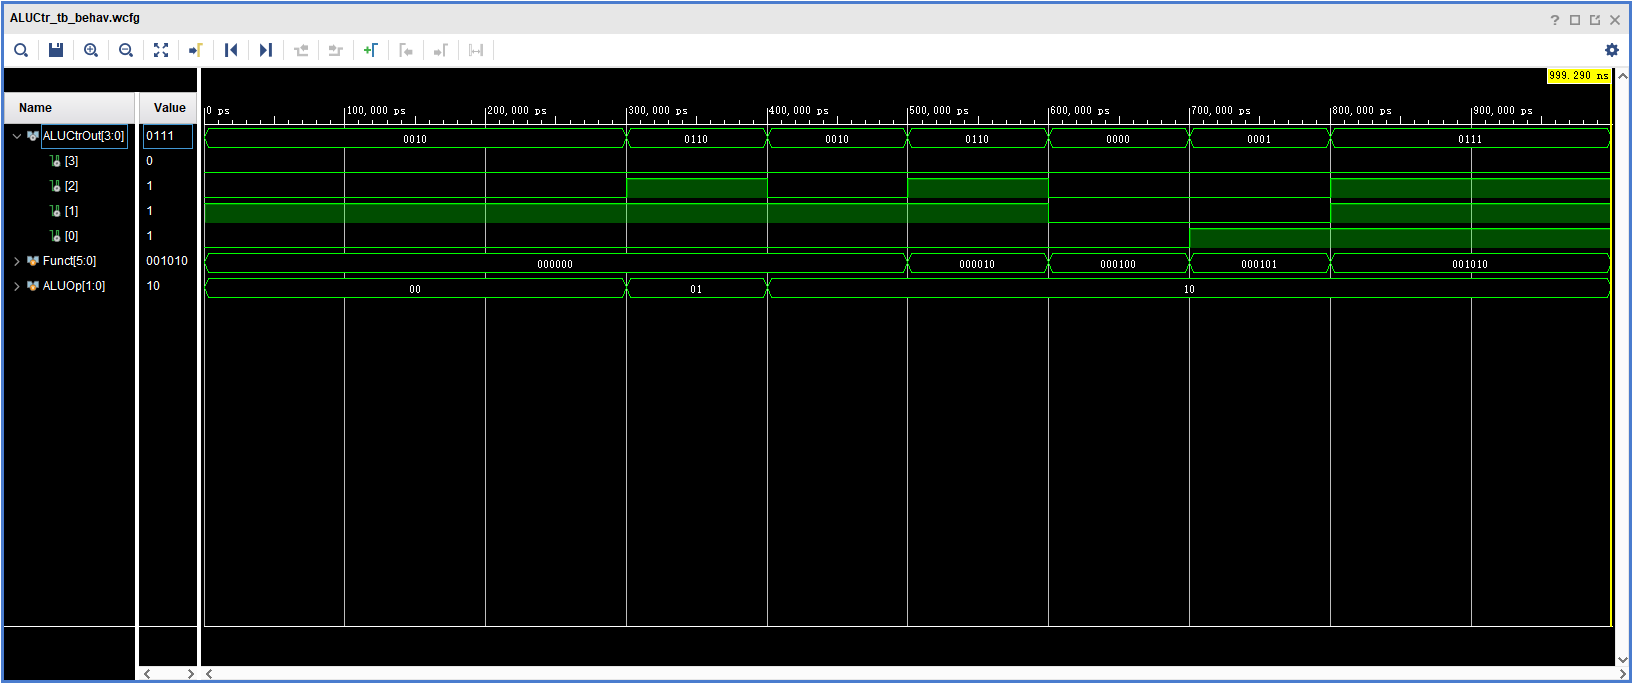
\includegraphics[width=\textwidth]{figure2.png}\caption{ALUCtr 仿真结果}\label{fig:aluctrtb}
\end{figure}

\subsection{ALU 模块}

ALU 模块的激励信号如下所示。
\begin{multicols}{2}
    \begin{lstlisting}[language=verilog,caption={ALU\_tb.v}]
    initial begin
    Input1 = 0;
    Input2 = 0;
    ALUCtr = 0;
    
    #100;
    Input1 = 15;
    Input2 = 10;

    #100;
    ALUCtr = 4'b0001;

    #100;
    ALUCtr = 4'b0010;

    #100;
    ALUCtr = 4'b0110;

    #100;
    Input1 = 10;
    Input2 = 15;

    #100;
    Input1 = 15;
    Input2 = 10;
    ALUCtr = 4'b0111;

    #100;
    Input1 = 10;
    Input2 = 15;

    #100;
    Input1 = 1;
    Input2 = 1;
    ALUCtr = 4'b1100;

    #100;
    Input1 = 16;
end
\end{lstlisting}
\end{multicols}


仿真结果如图 \ref{fig:alutb} 所示。完成了对应的功能。
\begin{figure}[H]
    \centering
    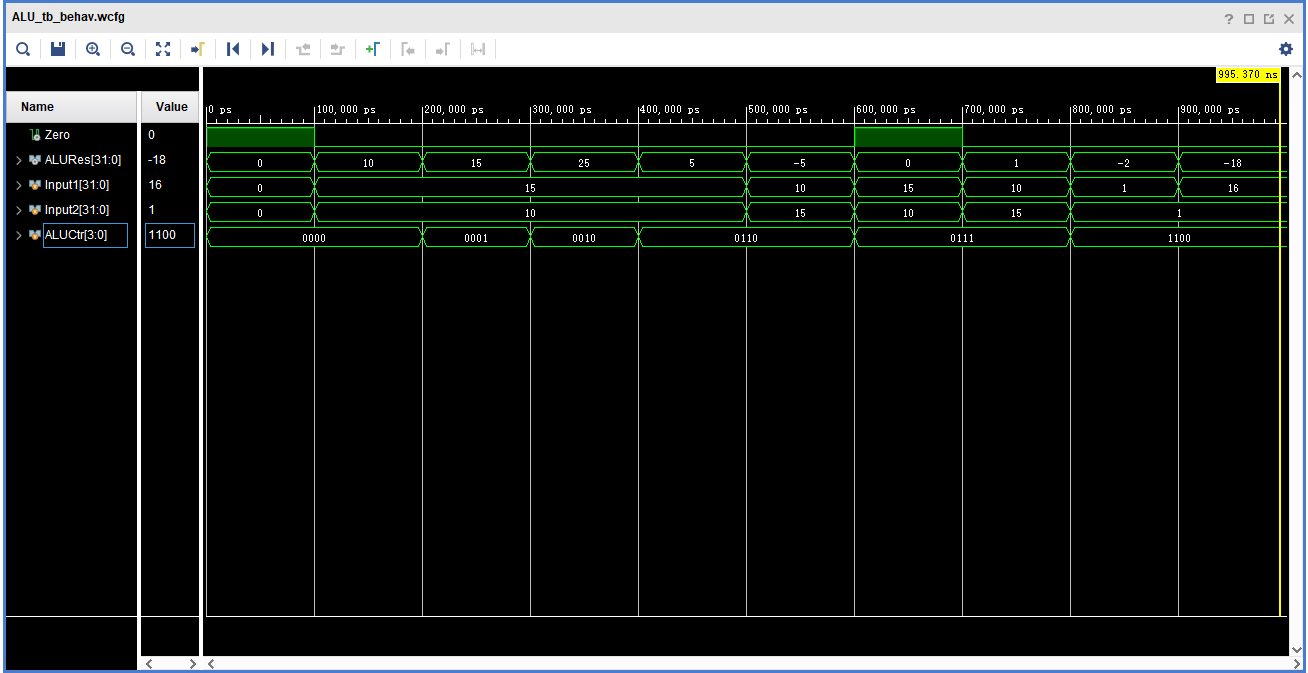
\includegraphics[width=\textwidth]{figure3.png}
    \caption{ALU 仿真波形}
    \label{fig:alutb}
\end{figure}

\section{实验心得}

本实验实现了 Ctr, ALUCtr, ALU 等模块,为之后的完整实现奠定了基础。通过本次实验,我熟悉了 Verilog 的相关语法(特别是 \verb"case" 和连接 \verb"{Op1,Op2}"),意识到在某些方面其与 C 语言的相似性(比如按位运算符)以及其 Visual Basic 类似的环境语法(\verb"begin",...,\verb"end"),熟悉了 模块编写 -- 激励编写 -- 仿真波形 -- 调试流程。熟悉了 MIPS 的译码和运算流程,对理解处理器结构很有帮助。

\end{document}